\chapter{Auslegung der Stromversorgung}

Um das Layout der Platine möglichst simpel zu halten und damit kostengünstig zu bleiben, wurden alle Komponenten so ausgewählt dass diese über eine einzige 5V Spannungsquelle mit Energie versorgt werden können.
Es wichtig den Stromverbrauch aller Komponenten abzuschätzten, um die Spannungsversorgung sinnvoll Dimensionieren zu können. Eine zu schwache spannungsquelle kann zu instabilitäten führen,
während eine überdimmensionierte Geld verschenkt.

\section{Stromverbrauch der Komponenten}
In diesem Abschnitt soll eine Abschätzung des Stromverbrauches vorgenommen werden. Dabei wird keinen Wert auf hohe Genauigkeit gelegt, es soll nur eine ungefäre Größenordnung für den Stromverbrauch gefunden werden.

\subsection{Servomotor}
Der Stromverbrauch des Servomotors ist schwer zu ermitteln, da es sich um einen Modellbauservomotor handelt 
sind im Datenbatt hierzu leider keine Daten aufzufinden. Da ein Messaufbau für die Abschätzung des Stromverbrauches
zu Aufwändig ist, werden hier Messwerte eines ähnlichen Servos aus einem Artikel \cite{website-servo} herangezogen.
Laut diesem hat eine Servomotor keinen konstanten Stromverbrauch. Der Stomfluss wird immerwieder unterbrochen, so das es zu einem Intervallartigen Stromfluss kommt.
Nur wenn der Servomotor dauerhaft belastet wird kommt es zu einem konstanten Stromfluss.
Im Artikel werden mehrere Servomotorn vermessen, der Motor der unserm am nächsten kommt ist der ``Graupner 4421'' mit folgenen Daten:

Technische Daten ``Graupner 4421'' \cite{website-servo-vergleich-dat}:
\begin{itemize}
 \item Stellzeit(60°): 0,11s
 \item Stellmoment: 88Ncm 
\end{itemize}


Technische Daten des verwendeten Servomotors \cite{website-servo-dat}:
\begin{itemize}
 \item Stellzeit(60°): 0,13s (4,8V) / 0,16s (6,0V)
 \item Stellmoment: 92Ncm (4,8V) / 78Ncm (6,0V)
\end{itemize}



Dieser hat laut des Artikels eine maximale Stromaufnahme von 1,2A. Um noch Luft nach oben zu haben wird hier ein Verbrauch von 
1,8A angenommen.

\subsection{Pandaboard ES}
Leider gibt es vom Hersteller des Pandaboards keine konkreten Angaben zum Stromverbrauch. Der Hersteller empfiehlt jedoch ein
Netzteil mit 4A\cite{website-panda-supply}, wobei auch ein Betrieb an USB mit hilfe eines Y-Kabels möglich ist. Die USB-2.0 Spezifikation\cite{website-usb-spec} sieht eine maximale 
Stromabgabe von 500mA vor.

Der Stromvebrauch des normalen Pandaboards (ohne ES) beträgt ca. 800mA \cite{website-panda-power}.
Nähere angaen zu Stromverbrauch des normalen Pandaboards (ohne ES) finden sich in \cite{website-panda-power}.
Der Verbrauchdes Pandaboard ES dürfte durch de Schnelleren Prozessor minimal darüber liegen. 
Durch anschluss von USB Geräten an dasBoard kann der Stomverbrauch jedoch noch steigen, Die USB-Spezifikation \cite{website-usb-spec}
sieht pro Port eine maximale Stomentnahme von 500mA vor. Da das Pandaboard über 2 USB ports verfügt liegt der maximale zusätzliche Verbrauch bei 1A
Sodas hier ein gesammt Verbrauch von 2A veranschalgt wird.

\subsection{Led Beleuchtung}
Auch wenn LEDs den Ruf haben besonders energieffizient zu sein ist der Stromerbrauch beieiner größeren anzahl nicht zu
unterschätzen. Da wir RBG-LEDs einsätzen besteht ein LED-Modul aus 3 LEDs in den Grundfarben rot, blau und grün.
Laut Datenblatt \cite{ds-WS2812} haben die LEDs eine Stromaufnahme von 20mA, also 60mA pro Modul.
Um Reglelwerk konform zu sein, werden folgende Beleuchtungen benötigt: Blinker rechts und links jeweils vorne und hinten.
Sowie eine leuchte welche din RC-Modus anzeigt. Zusätzlich zu denim Reglelwerk vorgeschriebenen Beleuchtungen werden noch
2 Frontscheinwerfer und Rückleuchten integriert. So dass sich eine Anzahl von 9 LED-Modulen ergibt.
Der maximale durch die LEDs verursachte Verbrauch liegt somit bei 540mA. 



Bremslichter???


\subsection{Microkontroller}
Der maximale Stromverbrauch des AVR Mikrocontrollers liegt laut Datenblatt\cite{ds-at90can} bei 200mA, wenn IO-Pins belastet werden
Der Mikrocontrollers selber braucht jedoch bei 5V Betriebsspauung und 16MHz nur 29mA. Da die IO-Pins des Controllers nur wenig belastet werden,
wird hier nur ein Verbrauch von 100mA veranschlagt.

\subsection{Sharp Sensoren}
Die Sharp GP2D120 distanz Sensoren liegt laut Datenblatt \cite{ds-sharp-GP2D120} bei 50mA, da 2 dieser Sensoren verbaut werden ergeben sich 100mA.

\subsection{Sonstige Peripherie}
Da der Stromverbrauch der restliche Komponenten minimal ist werden hier pauschal 100mA veranschalgt.

\section{Auswahl des Reglers}
Der Gesammtstromverbrauch der Komponenten beträgt 4.740mA. Ein Linearregler hier nicht mehr praktikabel, da dieser bei einer Akkuspannung von 14,4V und 3.740mA fast 45 Watt Leistung in Wärme umwandeln würde.
Eine gute Wahl für diesen Einsatzzweck ist der LM2678 von Texas Instruments, dieser kann dauerhaft einen Strom von 5A liefern und sein Wirkungsgrad liegt selbst bei maximallast bei über 80\%.
Eine Übersicht dazu findet sich in Abbildung [\ref{fig:vreg}].
\begin{figure}[H]
\centering
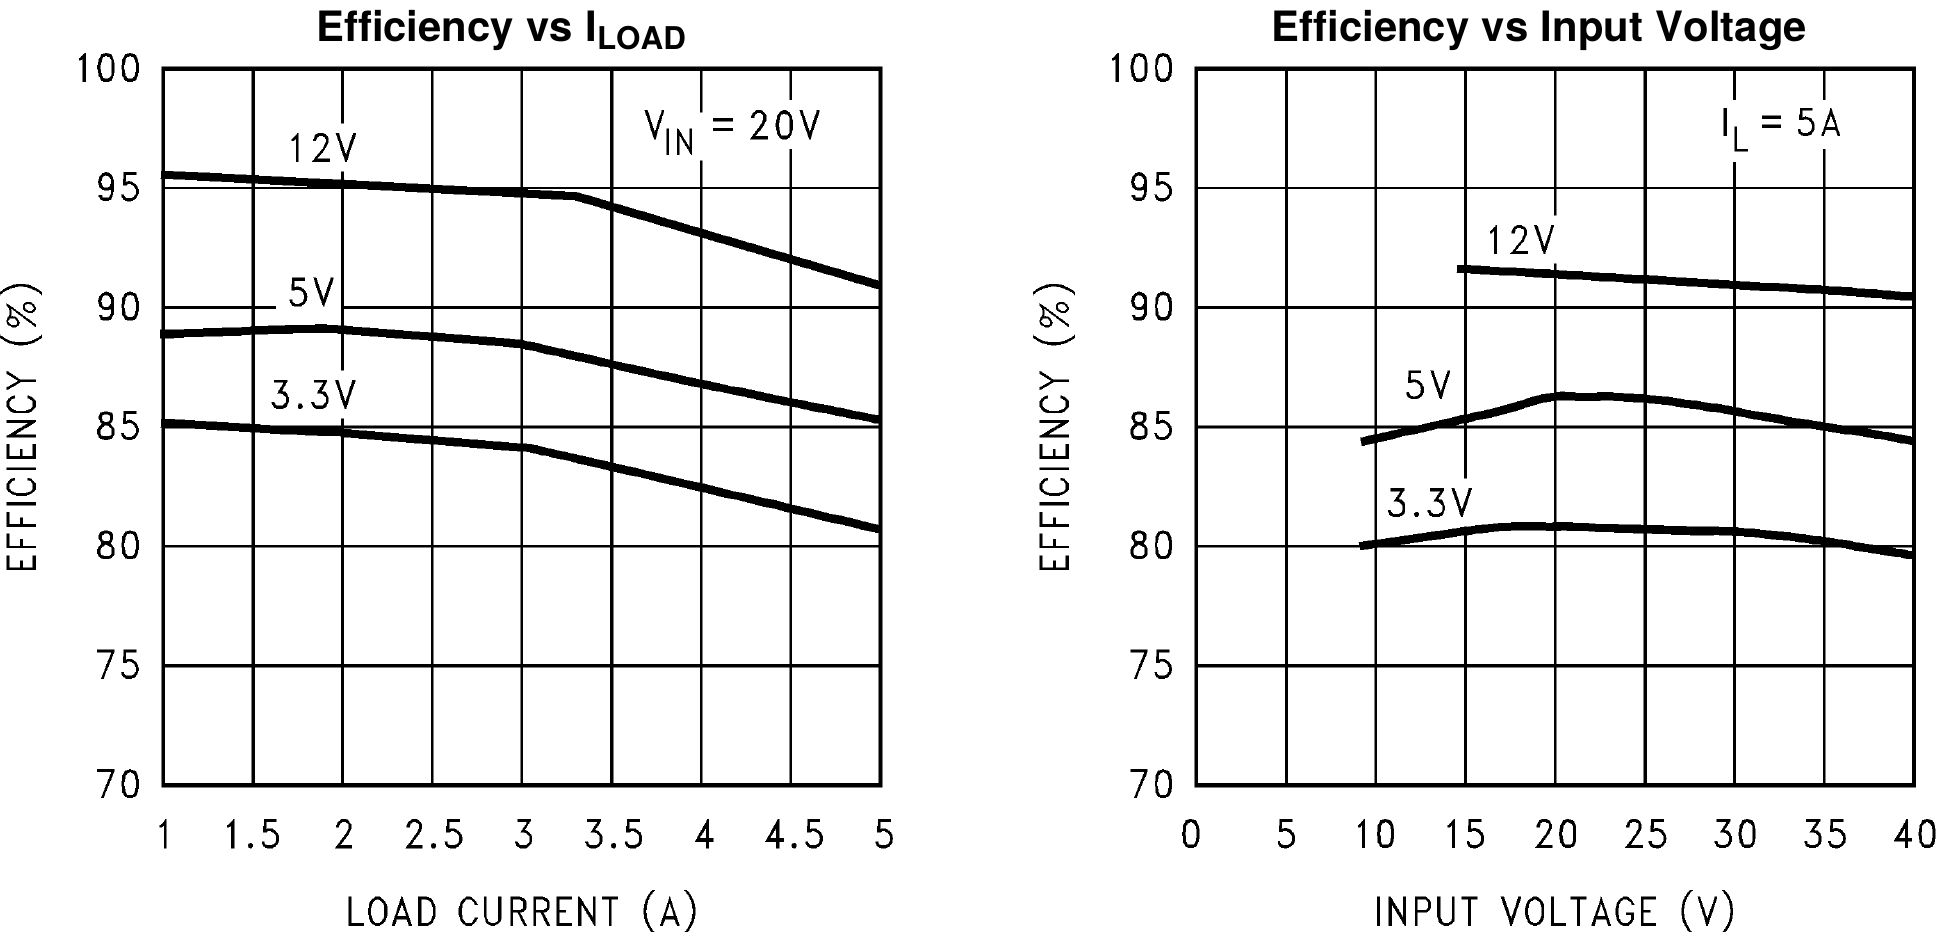
\includegraphics[width=.8\textwidth]{vreg.png}\\
\caption{Regulator Wirkungsgrad}%
\label{fig:vreg}
\end{figure}
Ausgehend von ca. 24 Watt Leistungsaufnahme ($4,8A*5V$) und einem minimalen Wirkungsgrad von 80\%  ergibt sich damit eine überschauliche Verlustleistung von 6 Watt.

